

\section{Tervezés}

\subsection{Bevezető}

Ebben a részben elsőként leírom, illetve összehasonlítom a multimédia üzenetküldő rendszer megvalósítási lehetőségeit, majd az általam kiválasztott módszer funkcionális egységeit,  részletesen tárgyalva azok szerepét és egymással való kapcsolatát.

\subsection{A megvalósítási lehetőségek}

Nézzük meg, hogy az IMS használata esetén milyen lehetőségek vannak a csoportos üzenetküldés megvalósítására. A megoldási lehetőségek ismertetése során kitérek azok előnyeire, hátrányaira, illetve a felmerülő problémákra.

\subsubsection{SIP MESSAGE üzenetek használata}
\label{sec:sip_message}

Első megoldásként kézenfekvőnek tűnhet, hogy a SIP protokoll által nyújtott MESSAGE típusú üzenet törzsében küldjük el a multimédia üzenetet a címzetteknek. Ennek a megoldásnak az az előnye, hogy nem kell másik protokollt használni az üzenetek átviteléért, hanem a SIP protokoll nyújtotta funkciókat alkalmazzuk. A megoldás előnye viszont eltörpül a hátrányok mellett. Először is a MESSAGE típusú üzenetnek nem adható meg egynél több címzett, így minden címzettnek különálló MESSAGE üzenetben kellene elküldeni ugyanazt a tartalmat. Ez a megszorítás redundanciához vezet, mivel a feladónak ugyanazt az üzenetet minden címzettnek külön-külön el kell küldenie, ami a válaszidőt is jelentősen megnöveli. Erre a problémára megoldást jelenthet, ha az üzenetet egy alkalmazás szerveren keresztül küldjük, ahol a szerver feladata az üzenet továbbítása az a címzetteknek. Ebben az esetben a feladó és a szerver között csak egyszer kerülne átküldésre az üzenet, ami a szűkebb sávszélességű felhasználói hálózatok esetén hatalmas előnyt jelent a többszörös küldéshez képest. Ahhoz, hogy ez a megvalósítás működhessen, a felhasználókból csoportokat kell létrehozni, és a MESSAGE üzenetet a címzettek URI-ja (Uniform Resource Identifier) helyett a csoport URI-jával címezni. Amikor az alkalmazás szerver megkapja ezt az üzenetet, a csoport azonosító alapján valamilyen módon -- pl. saját adatbázisból -- megkeresi azokat a felhasználókat, akik tagjai a csoportnak, és mindegyik csoporttagnak egyesével elküldi a kapott üzenet másolatát. Ebben az esetben szükség van az alkalmazás szerver oldalán egy olyan funkcióra, ami a csoportkezelést megvalósítja.
További problémát jelent, ha a küldött multimédia mérete meghaladja a MESSAGE üzenet törzsébe maximálisan megadható 1300 oktetet\footnote{RFC 3428 - Session Initiation Protocol Extension for Instant Messaging}. Ilyenkor a tartalmat a küldő oldalon kisebb darabokra kell tördelni, a darabokat külön üzenetekben elküldeni, majd a vevő oldalon a kisebb részekből a teljes üzenetet rekonstruálni. A probléma gyökere, hogy a SIP MESSAGE üzenettípus nem támogatja egy üzenet több darabban való átvitelét. A MESSAGE üzenet fejlécében nincs lehetőség olyan paramétert megadni, amiből a vevő egyértelműen el tudja dönteni, hogy a beérkező MESSAGE üzenetek közül melyik hordozza ugyanazon tartalom egy-egy darabját, és melyik nem, amiből következően rekonstruálni sem tudja azt. További gond, hogy az üzenetek nem sorszámozottak, így az eredeti küldési sorrendet sem tudnánk visszaállítani. Ezek a problémák abból fakadnak, hogy a MESSAGE üzenet használatát elsősorban rövid szöveges üzenetek továbbítására találták ki, és nem nagy multimédia tartalmakhoz. 
A megoldás hátrányainak sorát bővíti az is, hogy nem támogatott a késleltetett üzenetküldést sem. Utóbbi problémát -- hasonlóan a többszörös küldéshez -- orvosolhatnánk az alkalmazás szerver használatával, amely eltárolná azokat az üzeneteket, amelyek a nem elérhető címzetteknek mennek, és a szerver akkor kézbesítené azt, amikor a címzett elérhetővé válik.

{\color{red}(IDE MÉG RFC3428-ból PÁR DOLOG)
(Leírni még, hogy a vevők válasza többször jön, stb...)}

\subsubsection{Több címzettel rendelkező üzenetek használata}
\label{sec:mr_message}

Mint ahogy a \ref{sec:sip_message}.~fejezetben láthattuk, a SIP specifikáció nem nyújt hatékony megoldást a több címzettű üzenetek továbbítására. Ebben az alpontban leírt megoldás abban tér el az előzőhöz képest, hogy az üzenet fejlécben lehetőség van több címzettet megadni. A folytatásban az ilyen típusú üzenetet több címzettel rendelkező, azaz MR (Multi Recipient) üzenetnek fogom nevezni. A több címzett megadásának a lehetősége jelentős előnyt jelent az alap SIP MESSAGE-et használó megoldáshoz képest. Először is, a feladónak elég csak egyszer elküldeni az üzenetet a CSCF felé, és nem annyiszor, ahány címzettje van az üzenetnek. Ez jelentősen lecsökkenti a hálózati erőforrások használatát. Másodszor, mivel a címzettek az MR üzenet fejlécében helyezkednek el, így az erre alkalmas hálózati szerverek a fejléc adatokat felhasználva képesek az üzeneteket hatékonyan eljuttatni az összes címzettnek anélkül, hogy az üzenet törzsét meg kellene vizsgálniuk. Tegyük fel, hogy a feladó hálózatában lévő S-CSCF, miután megkapja feladótól az MR üzenetet, annak minden címzettjére meghatározza az adott címzett felé vezető következő állomást (next hop CSCF), ahová továbbítani kell azt. Abban az esetben, ha kettő vagy több címzett esetén ugyanaz a next hop, akkor az S-CSCF abba az irányba MR üzenetként küldi tovább az üzenetet. Ha minden címzett next hop CSCF-je különbözik egymástól, akkor a szerver az egyes next hop-oknak hagyományos üzenetben küldi el annak egy-egy másolatát. Mivel a hálózatban található összes CSCF hasonlóan viselkedik, mint a feladót kiszolgáló S-CSCF, ezzel a módszerrel két szerver között ugyanaz az üzenet pontosan egyszer kerül átvitelre. Az üzenet terjedésének folyamatát a \ref{fig:mrflow}.~ábrán követhetjük nyomon. Jól látható, hogy ezzel a módszerrel minden linken kizárólag egyszer küldjük át ugyanazt az üzenetet, ellentétben az aktuális IMS javaslattal, miszerint több címzett esetén egy linken többször kellene átküldeni ugyanazt az üzenetet (Például a III-as, IV-es és V-ös linken). Abban az esetben, ha egy olyan CSCF vesz egy MR üzenetet, amely nem képes MR üzeneteket kezelni, akkor a küldő CSCF felé hibaüzenetet küld. Ilyenkor a küldő CSCF újra elküldi az üzenetet hagyományos SIP üzenetként, minden címzettre külön-külön. 

\begin{figure}[htbp]
\center
\resizebox{10cm}{!}{
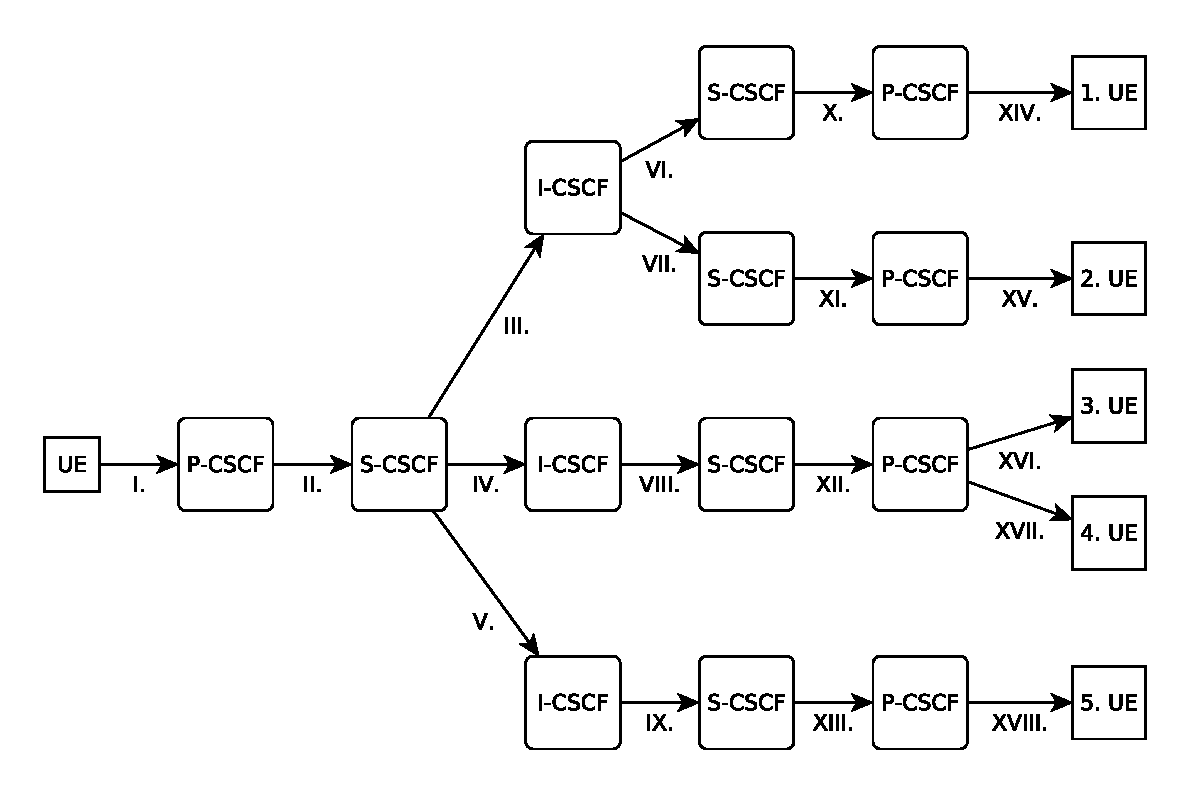
\includegraphics{img/MR-flow.eps}}
\caption{Az MR üzenetküldés folyamata}
\label{fig:mrflow}
\end{figure}

Mivel egy multimédia üzenet viszonylag nagy méretű is lehet, nagy valószínűséggel nem fér bele egyetlen MR üzenet törzsébe. Utóbbi probléma abból ered, hogy az IP hálózatokban maximalizálva van a hálózatba küldhető csomag mérete (MTU - Maximum Transmission Unit\footnote{IPV4-nél ez mekkora? Minimum 576 byte}). Hasonlóan a SIP MESSAGE üzeneteket használó megoldáshoz, itt is darabolni kellene a multimédia üzenetet több kisebb csomagra. Mivel az MR csomagok akár különböző útvonalon is eljuthatnak a címzettnek, a vételi oldalon való a csomagok eredeti sorrendjének visszaállíthatónak kell lennie. Amennyiben az MR üzenet fejlécében lehetőség lenne elhelyezni olyan mezőket, amelyek a helyes sorrend visszaállítását szolgálják, akkor a megoldás jelentősen jobb lenne, mint a SIP MESSAGE-et használó megvalósítás. Itt is általános feladatként jelentkezik a késleltett üzenetkézbesítés problémája, ami egy köztes alkalmazás szerver használatával megvalósítható lenne.

A vételi oldalon a kliensek, miután megkapták az MR kéréseket, nyugtázzák azokat. A cél itt is az, hogy a nyugták küldéséből eredő, a feladó és az őt kiszolgáló S-CSCF közötti linken folyó üzenetforgalmat minél jobban lecsökkentsük anélkül, hogy az IMS komponensek viselkedését alapvetően megváltoztatnánk. Ha a feladót kiszolgáló S-CSCF nem kompatibilis az MR üzenetekkel, akkor minden egyes nyugtát a hagyományos módon, egyesével továbbít a feladónak. Abban az esetben viszont, amikor az említett S-CSCF képes kezelni az MR üzeneteket, a hozzá beérkező, azonos típusú nyugtákra -- pl. 200 OK -- adott időtartamig vár, majd a nyugtákból összeállít egy MR választ, és csak ezt küldi el a feladónak, amivel jelentősen csökkenti a kérdéses link forgalmát.

\subsubsection{Üzenet továbbítása RTP protokoll segítségével -- {\color{red}IDE LEHET A VXML-es MRF-es megoldást kellene írni}}

{\color{red}Ezzel az a baj, hogy a video formátum erősen limitált. csak 3gp. Nem tudom, hogyan lehet képet átvinni. Ez főleg az interakciók miatt jó. max átvitt hang hossz is asszem limitált. Nem tudom, hogy erről kellene-e egyáltalán írni.}


\subsubsection{Üzenet továbbítása MSRP protokollal}
\label{sec:msrp_message}

Ez a megoldási javaslat a multimédia üzenetek felhasználók közötti átvitelére az MSRP (Message Session Relay Protocol) protokollt használja. Az MSRP -- a SIP-hez vagy a HTTP-hez hasonlóan -- egy szöveges, alkalmazás rétegbeli protokoll. A protokoll kapcsolat orientált adatátvitelt (session mode) tesz lehetővé, aminek számos előnye van a különálló, független üzenetcsomagok küldéséhez képest (paging mode).
Ezen előnyök közé tartozik, hogy a kommunikációs felek explicit felépítenek egymás között egy kommunikációs kapcsolatot az üzenet csomagok átvitelére. A kapcsolat léte magában foglalja többek között az összefüggő üzenet csomagok biztonságos, sorrendhelyes átvitelét, valamint a garantált kézbesítést is. Minden MSRP üzenet vagy egy kérés, vagy egy válasz. Az üzenetek fejlécből és törzsből állnak. A fejlécben az MSRP kapcsolatot, illetve a törzsben lévő -- szöveges vagy bináris -- tartalmat leíró információk találhatóak. Az MSRP kapcsolat felépítése SIP és SDP (Session Description Protocol) protokoll~\cite{rfc4566} segítségével történik. {\color{red} (IDE pár mondat az SDP-ről)} Az MSRP protokollról részletesebben az~\cite{rfc4975} irodalomban olvashat. 

Mivel a címzettek csoportjában lehet olyan felhasználó, aki az üzenet küldésének pillanatában nem elérhető, így a késletetett kézbesítés problémája ebben az esetben is felmerül. Utóbbi problémára itt is megoldást nyújt az, ha a kliensek közé egy alkalmazás szervert helyezünk el, amely többek között a késletetett üzenet kézbesítését is végzi. A köztes szerver használata a hálózati forgalmat is csökkenti, mivel a feladó és a szerver közötti, jellemzően alacsony sávszélességű (pl. rádiós) linken csak egyszer kerül átvitelre a -- gyakran nagy méretű -- multimédia üzenetet, szemben azzal az esettel, amikor a feladó minden címzettre külön-külön elküldi azt. Miután sikeresen átvitelre került a multimédia üzenet, a feladónak a címzettek listáját valamilyen módon, például egy SIP MESSAGE üzenet törzsében kézbesíteni kell a szerver felé. Mivel ez a lista jellemzően rövid szöveges üzenet, így belefér egyetlen SIP MESSAGE üzenetbe. A megoldás hátránya az MSRP kapcsolat felépítésének költsége, ami viszont a kapcsolat tényéből fakadó, már fentebb említett előnyökhöz képest elhanyagolható.

{\color{red} (... üzenet kézbesítés, előny, hátrány)}
\\
A dolgozatban a szolgáltatás fejlesztése során a fentebb leírt megoldások közül a legutolsó, MSRP protokollt használó megoldás használata mellett döntöttem. A SIP MESSAGE üzenetek használata nem célszerű a \ref{sec:sip_message}.~fejezetben leírt számos hátránya miatt. Az \ref{sec:mr_message}.~fejezetben tárgyalt MR üzenetet használó csoportos üzenetküldési megoldás jelenleg csak ajánlás formájában létezik, bárminemű szabványosítási eljárás jelenleg nincs folyamatban a témával kapcsolatban. Az MSRP protokollal való megvalósítás előnye a többi megoldási javaslattal szemben, hogy -- az IMS-ben jelen lévő --szabványosított eszközök használatára épít, illetve az adatátvitel kapcsolatorientált jellege eredményeként megbízható üzenetküldés valósítható meg. 

\subsection{Funkcionális terv}

A rendszer alapvetően a klasszikus kliens-szerver architektúrát valósítja meg. A kliensek azok, akik létrehozzák a multimédia üzeneteket, majd -- a szerver közvetítésével -- elküldik azt a kliensek egy általuk kiválasztott csoportjának. A szerver adatbázisban tárolja a multimédia üzenethez tartozó adatokat. A feladó kliens az átvitel sikerességéről folyamatos értesítést kap a szervertől. A szerver, miután sikeresen megkapta az új üzenetet, az elérhető címzetteket -- egy SIP MESSAGE üzenet törzsében -- azonnal értesíti erről. Az említett üzenet törzsének részletes felépítése az {\color{red}xyz fejezetben} található. 

A felhasználó, amikor egy üzenetek szeretne küldeni felhasználók egy adott csoportjának, első lépésként fel kell építenie egy MSRP kapcsolatot a szerver felé, amelyen keresztül a multimédia üzenet átvitelre kerül. Amikor az MSRP kapcsolat sikeresen felépült, a feladó a kapcsolaton keresztül MSRP üzenetek formájában elküldi a multimédia üzenetet a szervernek. Miután az üzenet sikeresen megérkezett a szerver oldalra, a feladó bontja az MSRP kapcsolatot a szerverrel. Ezután a felhasználó egy SIP MESSAGE típusú üzenet törzsében, jól definiált formátumban elküldi a szervernek a címzettek listáját, illetve opcionálisan egyéb, az elküldött multimédia üzenetre jellemző információt. Mivel ezen információk rövid szöveges formátumúak, beleférnek egyetlen SIP MESSAGE üzenetbe. Amikor a szerver sikeresen megkapta a listát is tartalmazó üzenetet, a multimédia tartalommal együtt adatbázisban eltárolja azt, majd nyugtázza a sikeres vételt a feladó felé. A szerver címzettek felé az alábbi módon kézbesítheti az üzenetet.

A rendszer a kliens-szerver architektúra szerint épül fel....

\begin{figure}[htbp]
\center
\resizebox{10cm}{!}{
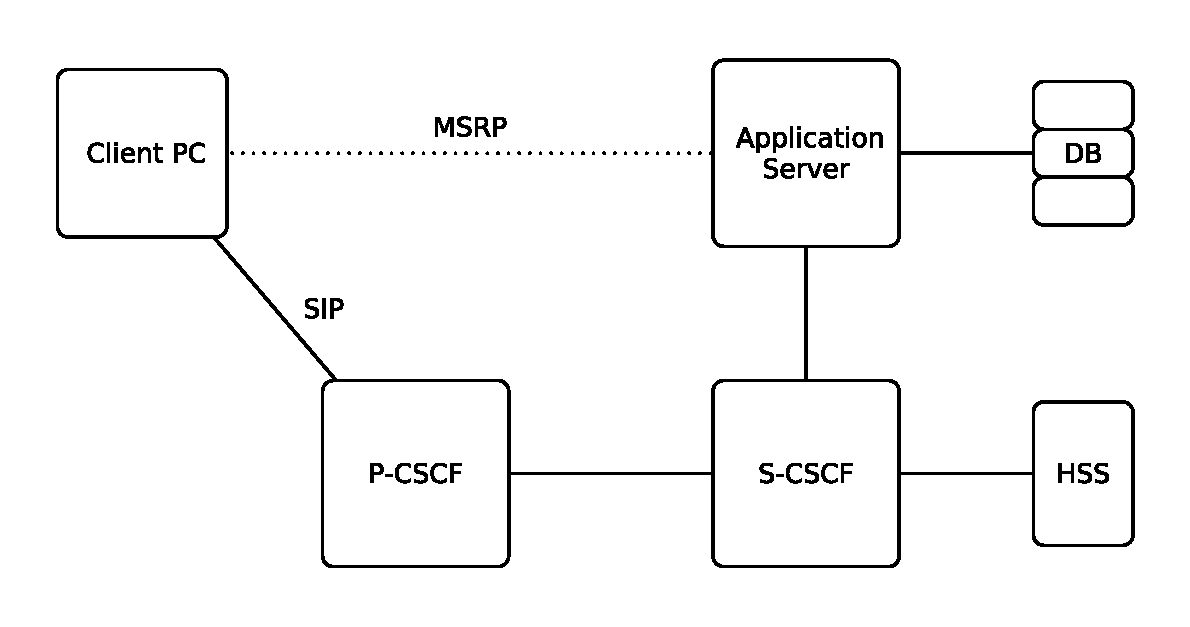
\includegraphics{img/system_MSRP_black.eps}}
\caption{A rendszer magasszintű modellje}
\label{fig:model}
\end{figure}


A következő fejezetekben az egyes elemek funkciójának részletes tárgyalása következik.

\subsubsection{Kliens}
\label{sec:kliens_pc}




\subsubsection{Alkalmazás szerver}
A megvalósítandó üzenetküldő rendszerben központi szerephet jut az alkalmazás szerver, ő végzi az üzenetek címzetteknek való szétosztását. A küldő kliens minden esetben az alkalmazás szerverrel építi fel a kapcsolatot, és annak küldi el a multimédia üzenetet. Két felhasználó közvetlenül soha nem küld egymásnak semmit. A szerver feladata kettős. Egyrészt fogadja a feladótól érkező multimédia üzenetet és továbbítja azt minden címzettnek külön-külön, másrészt a késletetett üzenettovábbítást valósítja meg. Utóbbi funkcióra akkor van szükség, ha a címzettek közül valamelyik nem elérhető. Ebben az esetben az AS akkor küldi el az üzenetet a címzettnek, amikor az elérhetővé válik.

\subsubsection{Adatbázis szerver}
\label{sec:adatbszerver}

A küldő felhasználótól az alkalmazás szerveren keresztül érkező üzenetek átmeneti tárolását valósítja meg. Egy adott üzenethez tartozó adatok mindaddig adatbázisban tárolódnak, amíg a szerver az összes címzetthez sikeresen nem továbbította az üzenetet, vagy valamely címzettek nem jelezték az alkalmazás szerver felé, hogy ők nem kívánják megkapni az adott multimédia üzenetet. Tárolásra kerülnek a feladótól érkező üzenet következő adatai:

\begin{itemize}\itemsep1pt
\item	A feladó SIP URI-ja
\item A címzettek SIP URI-jai
\item A üzenet azonosítója
\item Az üzenet tárgya
\item A multimédia tartalom
\item A multimédia tartalom formátuma
\end{itemize}

\subsubsection{Proxy CSCF}
\label{sec:p_cscf}

\subsubsection{Serving CSCF}
\label{sec:s_cscf}

\subsubsection{HSS}
\label{sec:hss}

\subsection{Üzemeltetési terv}
\label{sec:uzemeltetesi_terv}

Ide talán jöhetne use-case diagram, annak leírása...

\subsection{Interfész terv}
\label{sec:interfesz_terv}

Az egyes modulok közötti interfészek leírása...

Két fő komponensre különül el a rendszer fejlesztése: kliens-
ill. szerveroldali részre.

\subsubsection{Kliens}
\label{sec:kliensinterfesz}

\subsubsection{Szerver}
\label{sec:szerverinterfesz}

\subsection{Adatbázis terv}

A következő fejezetek a kommunikációs üzenetek szerkezetét valamint a használt adatbázis felépítését tárgyalják.


\subsubsection{Kommunikációs üzenetek}
\label{sec:kommuzenetek}

\subsubsection{Az adatbázis}
\label{sec:adatb}

\subsection{Megvalósítási terv}
\label{sec:megvalositas}

Ide jönnek majd az állapotgépek, működés leírása...

\subsubsection{A kliens megvalósítása}
\label{sec:kliensmegvalositas}

\subsubsection{A szerver megvalósítása}
\label{sec:szervermegvalositas}


\subsection{Összefoglalás}

